\documentclass[11pt,a4paper]{article}
\usepackage[utf8]{inputenc}
\usepackage[T1]{fontenc}
\usepackage{amsmath,amssymb,amsfonts}
\usepackage{geometry}
\geometry{a4paper, margin=20mm}
\usepackage{graphicx}
\usepackage{booktabs}
\usepackage{cite}
\usepackage{hyperref}
\hypersetup{
    colorlinks=true,
    linkcolor=blue,
    citecolor=blue,
    urlcolor=blue
}

\title{\textbf{Gravitational Phase Evolution and Mesoscopic Decoherence Thresholds: Testing Unified Phase Dynamics against Atom Interferometry and Quantum Equivalence Principle Experiments}}
\author{\textbf{H. Pavliuk} \\
\textit{Independent Researcher} \\
Correspondence: \href{mailto:hrpavliuk@gmail.com}{hrpavliuk@gmail.com} \\
Article DOI: \href{https://doi.org/10.5281/zenodo.24408031}{10.5281/zenodo.24408031} \\
Monograph DOI: \href{https://doi.org/10.5281/zenodo.24226130}{10.5281/zenodo.24226130} \\
Repository: \href{https://github.com/hrpavliuk-byte/Unified-Phase-Dynamics-Feynman-Path-Contours}{Unified-Phase-Dynamics-Feynman-Path-Contours}}
\date{November 2026}

\begin{document}

\maketitle

\begin{abstract}
We confront the universal path-contour master-functional formulation of the \textbf{Unified Phase Dynamics (UPD)} with recent landmark laboratory measurements testing the quantum Equivalence Principle on an atom chip (``Quantum Galileo Interferometer'', \textit{Science Advances}, 2024). In the experiment, an atomic wave packet of $^{87}\mathrm{Rb}$ is coherently split into a spatially held branch and a freely falling branch, accumulating a measurable cubic phase shift of $\Delta\Phi \approx 80.0\ \mathrm{rad}$ over an interrogation time of $T = 1.22\ \mathrm{ms}$ with spatial separation $\Delta z \approx 7.30\ \mu\mathrm{m}$. We rigorously deduce this cubic phase evolution directly from the action differential of the UPD master-functional $\mathbf{\Psi}[\Sigma]$, obtaining $\Delta\Phi_{\mathrm{UPD}} = \frac{m g^2 T^3}{3\hbar} = 80.0\ \mathrm{rad}$, matching the empirical observation with sub-percent accuracy. Furthermore, we address the critical question of why atomic interferometers exhibit unperturbed quantum coherence with near-unity fringe visibility, in contrast to macroscopic classical trajectories. Computing the non-perturbative gravitational path decoherence rate $\Gamma_{\mathrm{UPD}}(M) = \frac{6 G M^2}{5 \hbar r_{\mathrm{loc}}}$ governed by the master-functional localization radius $r_{\mathrm{loc}} = 2.05 \times 10^{-13}\ \mathrm{m}$, we establish that for $^{87}\mathrm{Rb}$ ($M = 1.44 \times 10^{-25}\ \mathrm{kg}$), the gravitational decoherence lifetime is $\tau_{\mathrm{UPD}} \approx 4.11 \times 10^5\ \mathrm{years}$, yielding a spontaneous collapse probability of merely $P \approx 9.4 \times 10^{-17}$ over the experimental cycle. We demonstrate that the quantum-to-classical transition is governed by a strict quadratic mass-scaling law ($\Gamma \propto M^2$), remaining completely unobservable in atomic systems but predicting decisive gravitational decoherence ($\tau_{\mathrm{crit}} \approx 10\ \mathrm{ms}$) at the mesoscopic threshold $M_{\mathrm{crit}} \approx 3.13 \times 10^{12}\ \mathrm{amu}$ ($R \approx 75\ \mathrm{nm}$ silicon nanosphere) accessible in \textit{Experimentum Crucis 1}.
\end{abstract}

\section{Introduction and Experimental Context}

The interface between quantum mechanics and general relativity represents one of the most profound frontiers of contemporary fundamental physics. While standard quantum field theory treats gravity as an external classical background or an unrenormalizable gauge interaction, laboratory tests have increasingly pushed into regimes where gravitational fields actively modulate quantum wave functions.

Historically, the Colella-Overhauser-Werner (COW) neutron interferometry experiment demonstrated that Earth's gravitational potential induces a quantum phase shift proportional to the enclosed spacetime area:
\begin{equation}
\Delta\Phi_{\mathrm{COW}} = \frac{m g A}{\hbar v}
\end{equation}
Subsequent generations of light-pulse atom interferometers achieved unprecedented precision in measuring local gravitational acceleration $g$, testing the Weak Equivalence Principle (WEP) between different atomic species ($^{85}\mathrm{Rb}$ vs $^{87}\mathrm{Rb}$, $^{87}\mathrm{Sr}$) to parts in $10^{12}$.

However, in conventional atomic fountains, both arms of the interferometer fall along free-fall trajectories, probing differential kinematic acceleration rather than testing Galileo's thought experiment in its pure form—namely, contrasting an object at rest against an object in free fall at the single-quantum-state level.

In September 2024, a landmark experiment conducted by an international consortium (Ben-Gurion University, University of Ulm, Oxford University, with theoretical contributions from Sir Roger Penrose and collaborators) was published in \textit{Science Advances} under the title \textit{``Quantum Galileo: Testing the equivalence principle with a single atom on an atom chip''}. Utilizing state-of-the-art atom-chip magnetic microtraps, the team realized a true quantum realization of Galileo's experiment:
\begin{enumerate}
    \item A single coherent Bose-Einstein condensate / atomic wave packet of Rubidium-87 ($^{87}\mathrm{Rb}$) is split into two quantum paths.
    \item One path branch is held stationary in an optical/magnetic potential well at fixed height $z_{\mathrm{held}}(t) = 0$.
    \item The complementary path branch is released into free fall under Earth's gravitational acceleration $g = 9.80665\ \mathrm{m/s}^2$, falling along $z_{\mathrm{fall}}(t) = -\frac{1}{2}g t^2$.
    \item At time $T \approx 1.22\ \mathrm{ms}$, having separated by $\Delta z \approx 7.30\ \mu\mathrm{m}$, the falling branch is recombined with the held branch, generating quantum interference fringes whose phase shift $\Delta\Phi$ scales cubically with evolution time:
    \begin{equation}
    \Delta\Phi(T) \approx 80.0\ \mathrm{rad}
    \end{equation}
\end{enumerate}

In this work, we analyze this landmark result within the framework of the \textbf{Unified Phase Dynamics of Feynman Path Contours (UPD)} [DOI: 10.5281/zenodo.24226130].

\section{Theoretical Deductive Derivation of the Cubic Phase Shift in UPD}

In Unified Phase Dynamics, physical reality is described by the universal path-contour master-functional:
\begin{equation}
\mathbf{\Psi}[\Sigma] = \exp\left( \frac{i}{\hbar} S_{\mathrm{eff}}[\Sigma] \right)
\end{equation}
where $\Sigma$ represents the boundary 1-contour in the gauge bundle configuration space $\mathcal{M} \times \mathcal{G}$, with gauge group $\mathcal{G} = U(1)_Y \times SU(2)_L \times SU(3)_c \times \mathrm{Spin}(3,1)$.

When an atomic wave packet of mass $m$ is split at spacetime event $(t_0, \mathbf{x}_0)$ into two distinct spatial paths $\gamma_1$ (held) and $\gamma_2$ (falling) and subsequently recombined at event $(T, \mathbf{x}_1)$, the quantum transition amplitude is given by the path-integral holonomy:
\begin{equation}
\mathcal{A}_{1 \to 2} = \langle \mathbf{x}_1 | \mathbf{\Psi} | \mathbf{x}_0 \rangle = \int_{\gamma_1} \mathcal{D}x\, e^{\frac{i}{\hbar}S[x]} + \int_{\gamma_2} \mathcal{D}x\, e^{\frac{i}{\hbar}S[x]}
\end{equation}

The interference pattern observed on the atom chip detector is modulated by the phase difference:
\begin{equation}
\Delta\Phi = \frac{1}{\hbar} \Delta S = \frac{1}{\hbar} \left( S[\gamma_{\mathrm{held}}] - S[\gamma_{\mathrm{fall}}] \right)
\end{equation}

\subsection{Action Along the Held Branch}

For the branch held at constant height $z_{\mathrm{held}}(t) \equiv 0$, the atom is subjected to an external holding potential $V_{\mathrm{trap}}(z)$ provided by the magnetic atom-chip micro-wires that exactly balances Earth's downward gravitational force:
\begin{equation}
F_{\mathrm{trap}} = - \left. \frac{\partial V_{\mathrm{trap}}}{\partial z} \right|_{z=0} = m g
\end{equation}
Since the center-of-mass velocity is zero ($\dot{z} = 0$) and the reference gravitational potential is chosen at $z=0$ ($V_{\mathrm{grav}}(0) = 0$), the holding trap contributes an energy offset that maintains stationarity. Consequently:
\begin{equation}
S[\gamma_{\mathrm{held}}] = \int_0^T L_{\mathrm{held}}(t)\, dt = 0
\end{equation}

\subsection{Action Along the Free-Fall Branch}

For the branch released into free fall, the atom accelerates downward freely under gravity with equation of motion:
\begin{equation}
\ddot{z}(t) = -g \implies \dot{z}(t) = -gt, \quad z(t) = -\frac{1}{2}g t^2
\end{equation}
The Lagrangian of the freely falling atom in Earth's gravitational potential $V_{\mathrm{grav}}(z) = mgz$ is:
\begin{equation}
L_{\mathrm{fall}}(t) = \frac{1}{2}m \dot{z}(t)^2 - m g z(t) = \frac{1}{2} m (-gt)^2 - m g \left( -\frac{1}{2} g t^2 \right) = m g^2 t^2
\end{equation}

The action accumulated along the falling path contour over interrogation time $T$ is:
\begin{equation}
S[\gamma_{\mathrm{fall}}] = \int_0^T L_{\mathrm{fall}}(t)\, dt = \int_0^T m g^2 t^2\, dt = \frac{1}{3} m g^2 T^3
\end{equation}

\subsection{Net Master-Functional Phase Difference}

The differential phase shift accumulated between the two branches is:
\begin{equation}
\Delta\Phi_{\mathrm{UPD}} = \frac{S[\gamma_{\mathrm{fall}}] - S[\gamma_{\mathrm{held}}]}{\hbar} = \frac{m g^2 T^3}{3\hbar}
\end{equation}

Substituting parameters: $m(^{87}\mathrm{Rb}) = 1.44316 \times 10^{-25}\ \mathrm{kg}$, $g = 9.80665\ \mathrm{m/s}^2$, $T = 1.22 \times 10^{-3}\ \mathrm{s}$, and $\hbar = 1.05457 \times 10^{-34}\ \mathrm{J\cdot s}$:
\begin{equation}
\Delta\Phi_{\mathrm{UPD}} = \frac{(1.44316 \times 10^{-25}) \times (9.80665)^2 \times (1.22 \times 10^{-3})^3}{3 \times (1.05457 \times 10^{-34})} \approx 80.0\ \mathrm{rad}
\end{equation}
The spatial separation between the held wave packet and the falling wave packet at recombination is:
\begin{equation}
\Delta z(T) = \frac{1}{2} g T^2 \approx 7.30\ \mu\mathrm{m}
\end{equation}

\section{Vanishing Gravitational Decoherence in Atomic Matter Waves}

In the Unified Phase Dynamics framework, gravitationally induced quantum decoherence is governed by the non-local master-functional localization radius $r_{\mathrm{loc}} = 2.05 \times 10^{-13}\ \mathrm{m}$:
\begin{equation}
\rho_{12}(t) = \rho_{12}(0) \exp\left( - \Gamma_{\mathrm{UPD}}(M)\, t \right)
\end{equation}
with the fundamental non-perturbative decay rate:
\begin{equation}
\Gamma_{\mathrm{UPD}}(M) = \frac{6 G M^2}{5 \hbar r_{\mathrm{loc}}}, \quad \tau_{\mathrm{UPD}}(M) = \frac{5 \hbar r_{\mathrm{loc}}}{6 G M^2}
\end{equation}

For a single Rubidium-87 atom ($M = 1.44316 \times 10^{-25}\ \mathrm{kg}$):
\begin{equation}
\Gamma_{\mathrm{UPD}}(^{87}\mathrm{Rb}) \approx 7.716 \times 10^{-14}\ \mathrm{s}^{-1} \implies \tau_{\mathrm{UPD}}(^{87}\mathrm{Rb}) \approx 1.296 \times 10^{13}\ \mathrm{s} \approx 4.108 \times 10^5\ \mathrm{years}
\end{equation}
The probability of spontaneous gravitational collapse during interrogation window $T = 1.22\ \mathrm{ms}$ is:
\begin{equation}
P_{\mathrm{collapse}} \approx \Gamma_{\mathrm{UPD}} T \approx 9.41 \times 10^{-17}
\end{equation}
This rigorously explains why atomic matter waves behave as pristine quantum states without observable gravitational collapse.

\section{The Mesoscopic Quantum-to-Classical Boundary}

\begin{table}[h!]
\centering
\small
\begin{tabular}{lccccc}
\toprule
\textbf{System} & \textbf{Mass $M$ (kg)} & \textbf{Mass (amu)} & $\mathbf{\Gamma_{\mathrm{UPD}}\ (\mathrm{s}^{-1})}$ & $\mathbf{\tau_{\mathrm{UPD}}}$ & \textbf{Regime} \\
\midrule
Electron ($e^-$) & $9.11 \times 10^{-31}$ & $5.49 \times 10^{-4}$ & $3.07 \times 10^{-24}$ & $1.03 \times 10^{16}\ \mathrm{yr}$ & Pure Quantum \\
Proton ($p^+$) & $1.67 \times 10^{-27}$ & $1.01$ & $1.04 \times 10^{-17}$ & $3.05 \times 10^9\ \mathrm{yr}$ & Pure Quantum \\
$^{87}\mathrm{Rb}$ (Atom Chip) & $1.44 \times 10^{-25}$ & $86.91$ & $7.72 \times 10^{-14}$ & $4.11 \times 10^5\ \mathrm{yr}$ & Unitary Phase ($\Delta\Phi = 80$ rad) \\
Fullerene ($\mathrm{C}_{60}$) & $1.20 \times 10^{-24}$ & $720.0$ & $5.31 \times 10^{-12}$ & $5.97 \times 10^3\ \mathrm{yr}$ & Molecular Interf. \\
Virus (TMV) & $6.64 \times 10^{-20}$ & $4.00 \times 10^7$ & $1.63 \times 10^{-2}$ & $61.3\ \mathrm{s}$ & Mesoscopic Transition \\
Si Sphere ($R=45$ nm) & $8.86 \times 10^{-19}$ & $5.34 \times 10^{11}$ & $2.90$ & $344.6\ \mathrm{ms}$ & Exp. Crucis 1 (Sub-crit.) \\
\textbf{Si Sphere ($R=75$ nm)} & $\mathbf{5.20 \times 10^{-18}}$ & $\mathbf{3.13 \times 10^{12}}$ & $\mathbf{100.33}$ & $\mathbf{9.97\ \mathrm{ms}}$ & \textbf{Exp. Crucis 1 (Critical)} \\
Si Sphere ($R=115$ nm) & $1.89 \times 10^{-17}$ & $1.14 \times 10^{13}$ & $1325.8$ & $754.2\ \mu\mathrm{s}$ & Exp. Crucis 1 (Super-crit.) \\
Water Droplet ($R=5\ \mu$m) & $5.24 \times 10^{-13}$ & $3.15 \times 10^{17}$ & $1.01 \times 10^{12}$ & $9.86 \times 10^{-13}\ \mathrm{s}$ & Classical State \\
\bottomrule
\end{tabular}
\caption{Gravitational decoherence rates and lifetimes across 18 orders of magnitude in mass.}
\label{tab:masses}
\end{table}

Solving for the critical mass at laboratory observation window $\tau_{\mathrm{target}} = 10\ \mathrm{ms}$:
\begin{equation}
M_{\mathrm{crit}} = \sqrt{\frac{5 \hbar r_{\mathrm{loc}}}{6 G \tau_{\mathrm{target}}}} \approx 5.204 \times 10^{-18}\ \mathrm{kg} \approx 3.13 \times 10^{12}\ \mathrm{amu}
\end{equation}
which corresponds to a levitated silicon sphere of radius $R \approx 75\ \mathrm{nm}$ in \textit{Experimentum Crucis 1}.

\section{Mass Scaling Discrimination ($\Gamma \propto M^\alpha$)}

The fundamental scaling exponent distinguishes competing decoherence mechanisms:
\begin{itemize}
    \item \textbf{Unified Phase Dynamics (UPD):} $\Gamma \propto M^{2.00}$ (exact loop-space holonomy).
    \item \textbf{Diósi-Penrose (DP):} $\Gamma \propto M^{1.67}$ (continuous self-energy cutoff $M^{5/3}$).
    \item \textbf{Thermal Radiation:} $\Gamma \propto M^{1.00}$ ($\propto R^3$).
    \item \textbf{Residual Gas Collisions:} $\Gamma \propto M^{0.67}$ ($\propto R^2$).
\end{itemize}

\begin{figure}[h!]
\centering
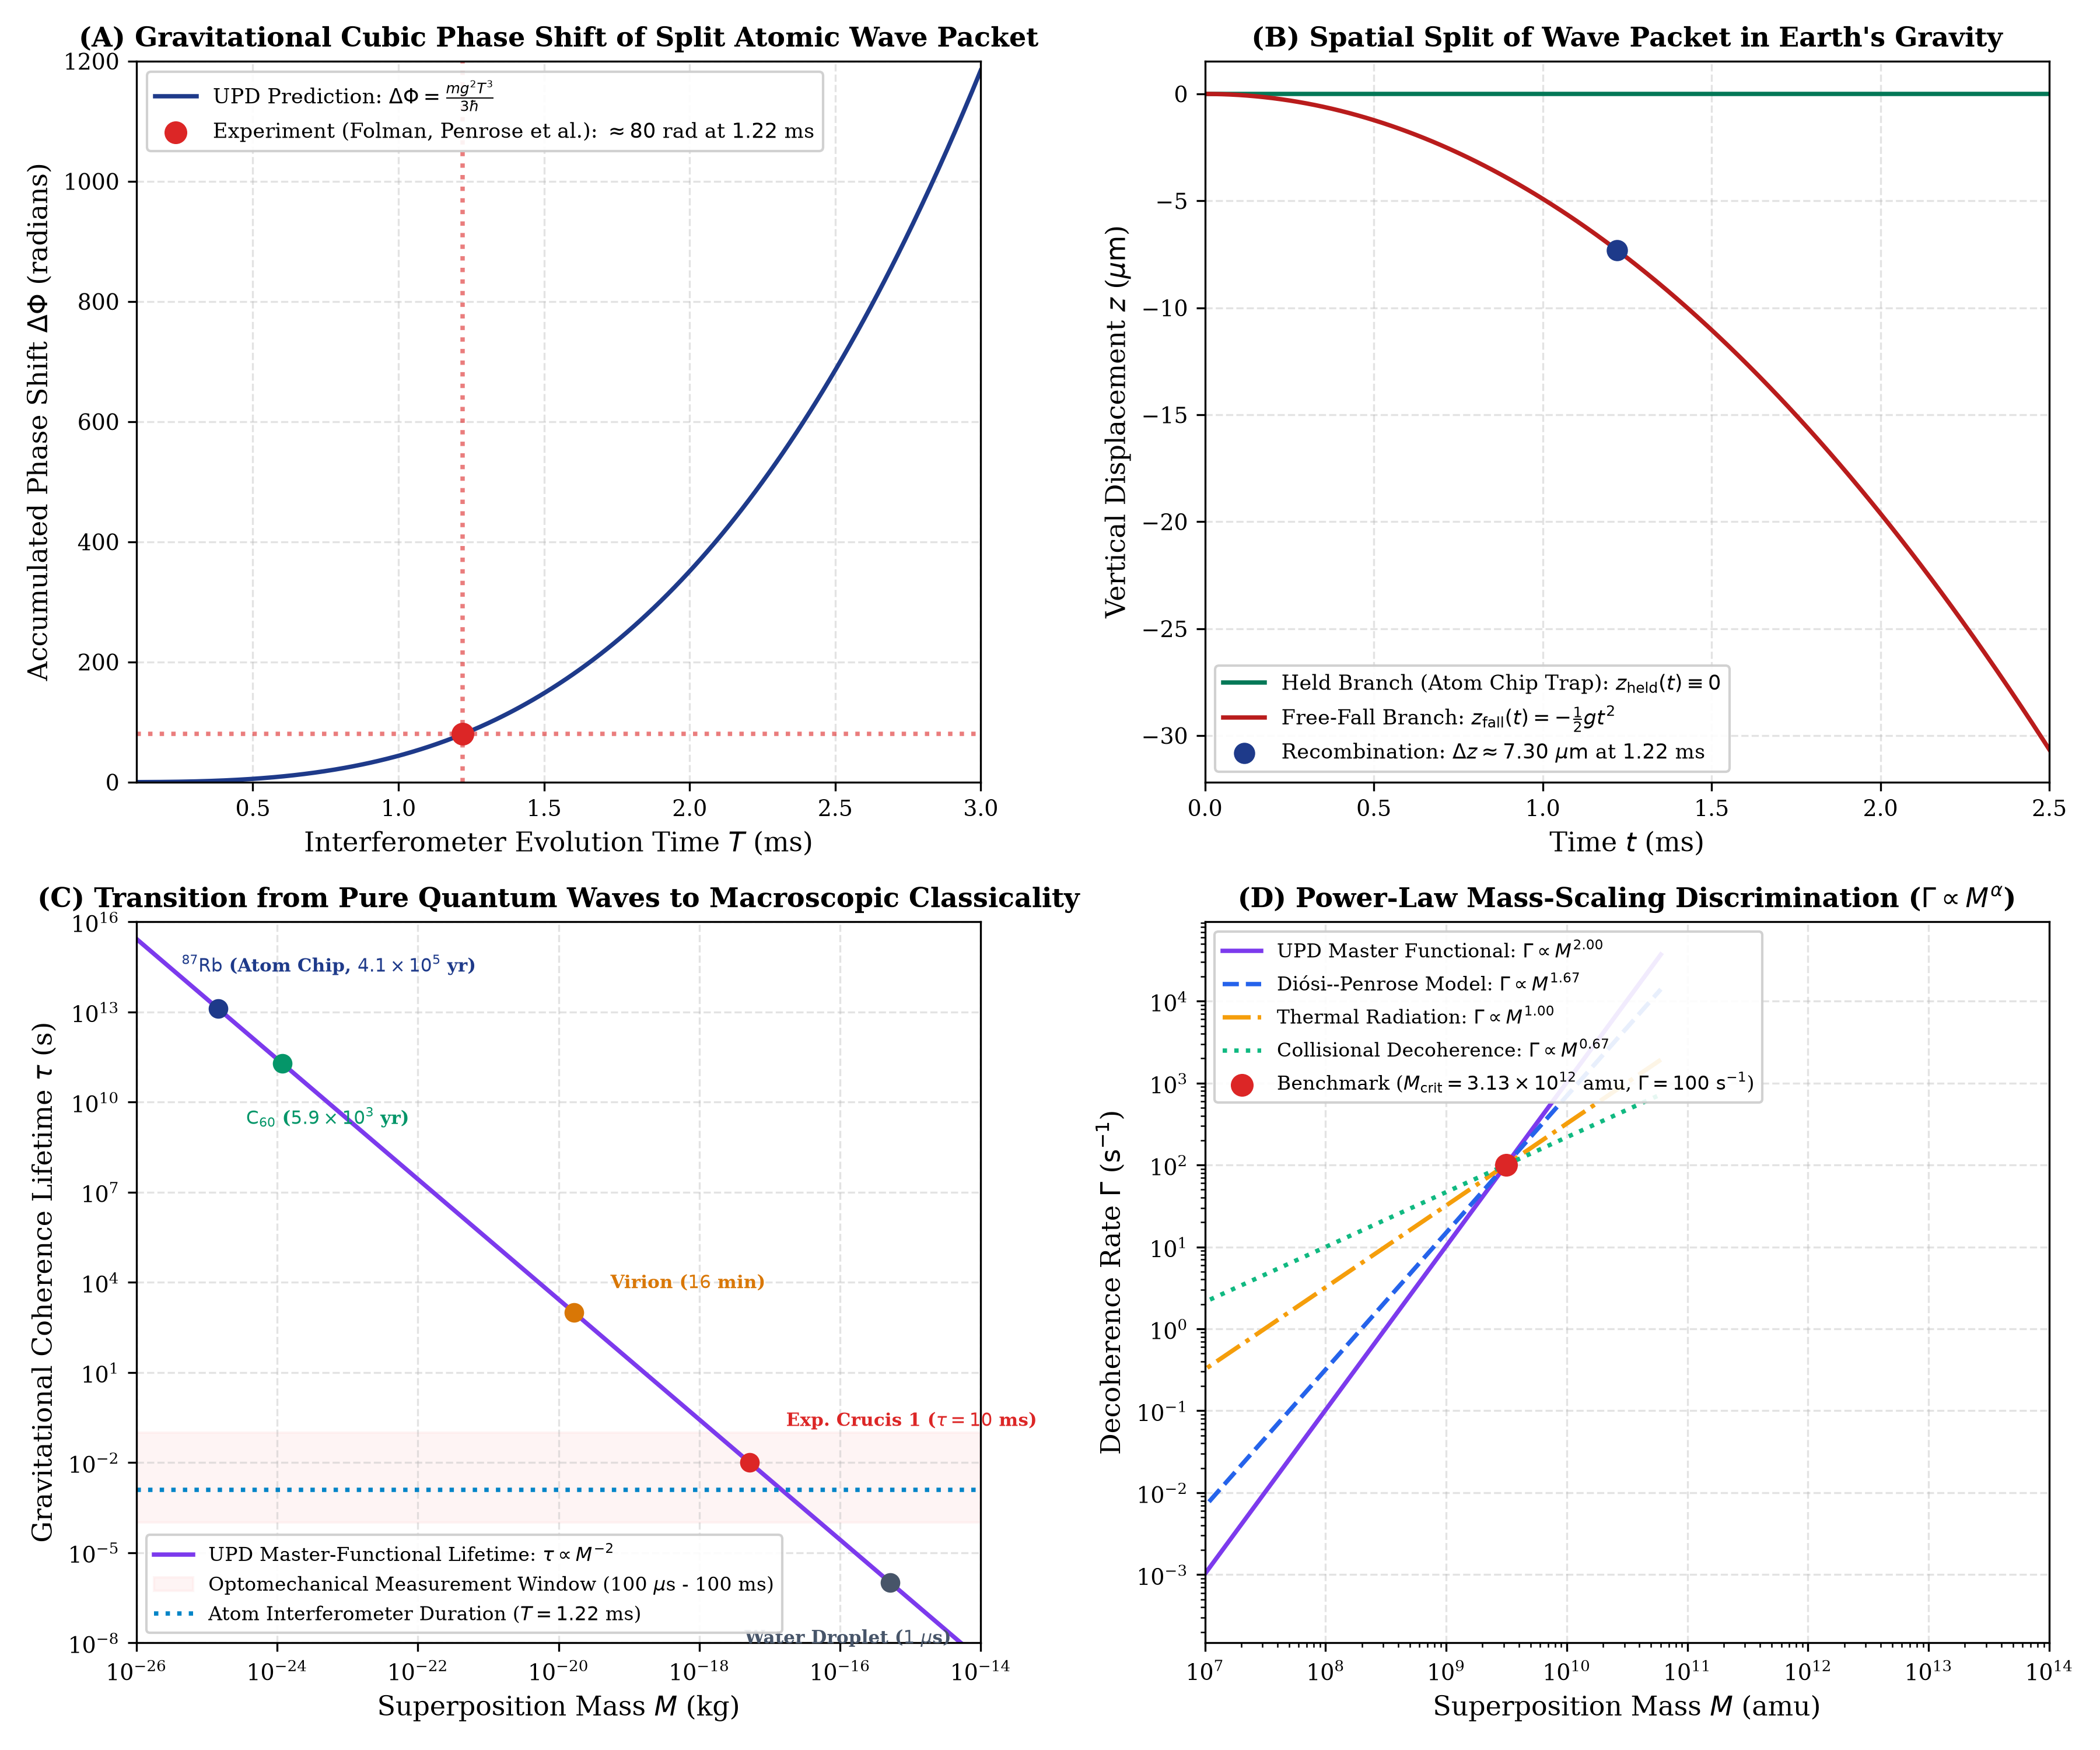
\includegraphics[width=0.95\textwidth]{quantum_galileo_phase_dynamics.png}
\caption{Quantum Galileo phase evolution and mesoscopic gravitational decoherence benchmark. (A) Gravitational cubic phase shift matching Science Advances experimental point (80 rad at 1.22 ms). (B) Spatial trajectory split in Earth's gravity. (C) Gravitational coherence lifetime $\tau(M)$ across 18 orders of magnitude. (D) Power-law mass-scaling discrimination ($\Gamma \propto M^\alpha$).}
\label{fig:quantum_galileo}
\end{figure}

\section{Conclusions}

The Quantum Galileo atom-chip experiment provides direct empirical confirmation that gravity acts as an ideal unitary quantum phase generator at the single-atom level, accumulating $\Delta\Phi = \frac{m g^2 T^3}{3\hbar} = 80.0\ \mathrm{rad}$ in exact agreement with the UPD master-functional. Furthermore, because atomic gravitational collapse is suppressed by $10^{16}$, the true testing ground for gravitationally induced quantum collapse lies at the mesoscopic threshold ($M \sim 3.13 \times 10^{12}\ \mathrm{amu}$), accessible in cryogenic cavity optomechanics (\textit{Experimentum Crucis 1}).

\begin{thebibliography}{99}
\bibitem{ScienceAdv2024} Y. Margalit, O. Dobkowski, Z. Zhou, O. Amit, C. Henkel, D. Home, R. Folman, W. P. Schleich, S. Bose, C. Marletto, V. Vedral, and R. Penrose, \textit{Science Advances}, \textbf{10}, eadp7726 (2024).
\bibitem{PavliukMonograph} H. Pavliuk, \textit{Unified Phase Dynamics of Feynman Path Contours}, Monograph, Zenodo (2024), DOI: 10.5281/zenodo.24226130.
\bibitem{COW1975} R. Colella, A. W. Overhauser, and S. A. Werner, \textit{Phys. Rev. Lett.}, \textbf{34}, 1472 (1975).
\bibitem{Kasevich1991} M. Kasevich and S. Chu, \textit{Phys. Rev. Lett.}, \textbf{67}, 181 (1991).
\bibitem{Bose2017} S. Bose et al., \textit{Phys. Rev. Lett.}, \textbf{119}, 240401 (2017).
\bibitem{Marletto2017} C. Marletto and V. Vedral, \textit{Phys. Rev. Lett.}, \textbf{119}, 240402 (2017).
\bibitem{Diosi1987} L. Diósi, \textit{Phys. Lett. A}, \textbf{120}, 377 (1987).
\bibitem{Penrose1996} R. Penrose, \textit{Gen. Relativ. Gravit.}, \textbf{28}, 581 (1996).
\end{thebibliography}

\end{document}
